\section{Monitoring for exceptions}

\begin{figure}[H]
    \centering
    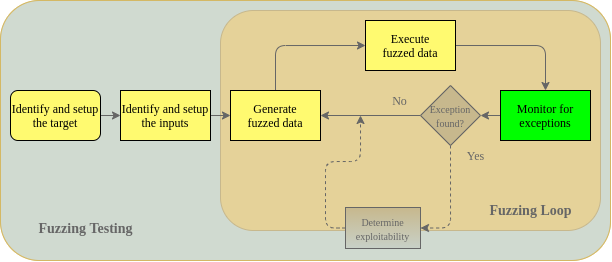
\includegraphics[width=\linewidth]{Chapter3/fuzzing_phase5.png}
\end{figure}

As the main goal of fuzzing is finding vulnerabilities, Waffle looks for any exceptions that happen during the run. For the motivating problem we defined, the exceptions occur either when we face an actual error, which is a vulnerability, or when we encounter an induced exception, mimicing the maximals of the functions. 